
% summary of this section.
In this section we highlight the importance of this case study has for embedded
software in safety-critical systems, and how SyVolt can contribute to the
development of these.

Then we give a number of semantic and syntactic contracts we wish to prove on the transformation described in Section~\ref{sec:mbeddr_transformation}. We end the section with some discussion about the limits of the SyVOLT contract language




\subsection{Correct Embedded Systems}

% Embedded systems need to be reliable.
The main reason for us to choose this case study is that embedded systems need
to be reliable: there are industry standards such as ISO-26262, DO-178B or
IEC-61508 to help ensure reliability and there are critical embedded systems
such as pacemakers \cite{mry_et_al:DR:2014:4543} that must be shown to be
correct.

% Traditional development of reliable embedded systems
Traditionally, embedded systems are implemented in C code and reliability is
ensured by a combination of testing and formal verification techniques such as
model checking. However, testing only guarantees reliability in as far as the
test cases go, and achieving the necessary high coverage is a lot of work.
Model checking, on the other hand, is very expensive because of C's high
expressivity and the resulting state space explosion problem. In order to
properly apply model checking techniques \cite{Ivancic2005}.
The abstraction process is error prone and time consuming as is described in
\cite{Corbett2000} and \cite{Ratiu:2012:LEE:2663689.2663692}.

% Mbeddr contribution to the reliable embedded systems development
mbeddr represents an evolution of traditional embedded system development
because it starts with abstractions that can be proven to be
correct\markus{That's probably a bit strong. Let's discuss how to say this
better} and then generates C code.
Model checking techniques can be applied to mbeddr models because they contain
higher level information (e.g., state machines, decision tables or contracts on
interface) whereas with plain C code, these abstractions need to be inferred
from the C.

% how does mbeddr help ensure correct embedded systems
\markus{This is no longer true. We use Sat4J and CBMC.}
% mbeddr is integrated with the NuSMV~\cite{Cimatti2002} model checker to perform
% model checking of the state machines and with the Yices~\cite{Dutertre:cav2014}
% Satisfiability Modulo Theories (SMT) solver to check the consistency and
% completeness of the decision tables.

% properties vs contracts
It is important to distinguish two types of properties: properties that a given
mbeddr model needs to satisfy; and properties that all mbeddr models need to
satisfy. For instance, a property of the former type for the mbeddr model of the
pacemaker system is that it never stops. A property of the later type is that
decision tables, if they are used, must be consistent and
complete~\cite{Ratiu:2012:LEE:2663689.2663692} or that contracts expressed on
interfaces are fulfilled by all implementing components.

% the problems with mbeddr level of abstraction
As described in~\cite{Ratiu:2012:LEE:2663689.2663692}, properties checked at the
mbeddr level can only be sound if the C code that is generated satisfies the
same properties as the mbeddr models. It is this crucial to achieve soundness of
the transformations from mbeddr's abstractions down to C. In practice this
correctness is ensured by manual reviews of the code generation and
lots of automated tests.

% how can syvolt help to ensure reliability
SyVolt is a step towards ensuring the C code generation is \emph{always}
correct, provided the appropriate correctness properties (of the C code
generation) are described. SyVolt allows the the transformation developer to
express contracts that relate the generated C construct to the constructs
available as extensions. This is something that cannot be done by checking the
generated C code alone as it requires the traceability information between the
generated C code and the mbeddr model\markus{This last sentence seems oddly
out of place. Why is this trace stuff relevant here?}.

% example
\markus{Is this merely an example, or is this THE CASE STUDY? I thiink the
latter. Rephrase?} For instance, in SyVolt it is possible to prove that the
wiring of instances of components is always translated to C correctly, i.e.,
when executing the C code, no instance will invoke a different operation than
the one that is specified in the wiring scheme at the mbeddr components level.
This is an important contract as it ensures, for instance, that the Client
component instance in our Client/Server example (see
Listing~\ref{code:simple_example_mbeddr}) will never invoke the operation of the
BadServer component instance.

To see how non-trivial this contract can be, look at the wiring function
\verb=client_wire= of the generated code from the Client/Server example shown in
Listing~\ref{code:components_sample_c}: the wiring in the C code is done by
assignment the address of the required port operation to a function pointer that
is part of the instance's runtime data.\cgg{I must stress this complexity by
explaining better how the wriring is done and how the function is then called.
Relying on the reader to understand this complexity from the example is
non-sense.}\markus{In particular, it is important to explain WHY the pointer
indirection is used: to support polymorphism} For more complex examples, this
becomes very difficult to inspect in the generated code\markus{But we don't
verify because it is hard to inspect, because after all, we can simply run a
test. We verify because we want a Proof!}.



\subsection{Correct Code Generation}

% pre-requisites for correctness.

In order for the transformation we just described to be correct, the wiring of
instances must be correct. The pre-requisites for this are:

\begin{compactenum}

\item The pointers to the provided port operations, assigned to the instance
variable that requires those operations do really point to the corresponding
operations.

\item The correct pointers are assigned to the correct instance variable.

\item Besides in the wiring function, that is called by the initialization
function, the instance variables' member that contains the provided port
operation reference is not assigned anywhere else.

\item The same thing as the previous for the pointers.
\end{compactenum}



\subsection{Contract 1: AssignmentInstance}

\begin{figure}
\begin{center}
  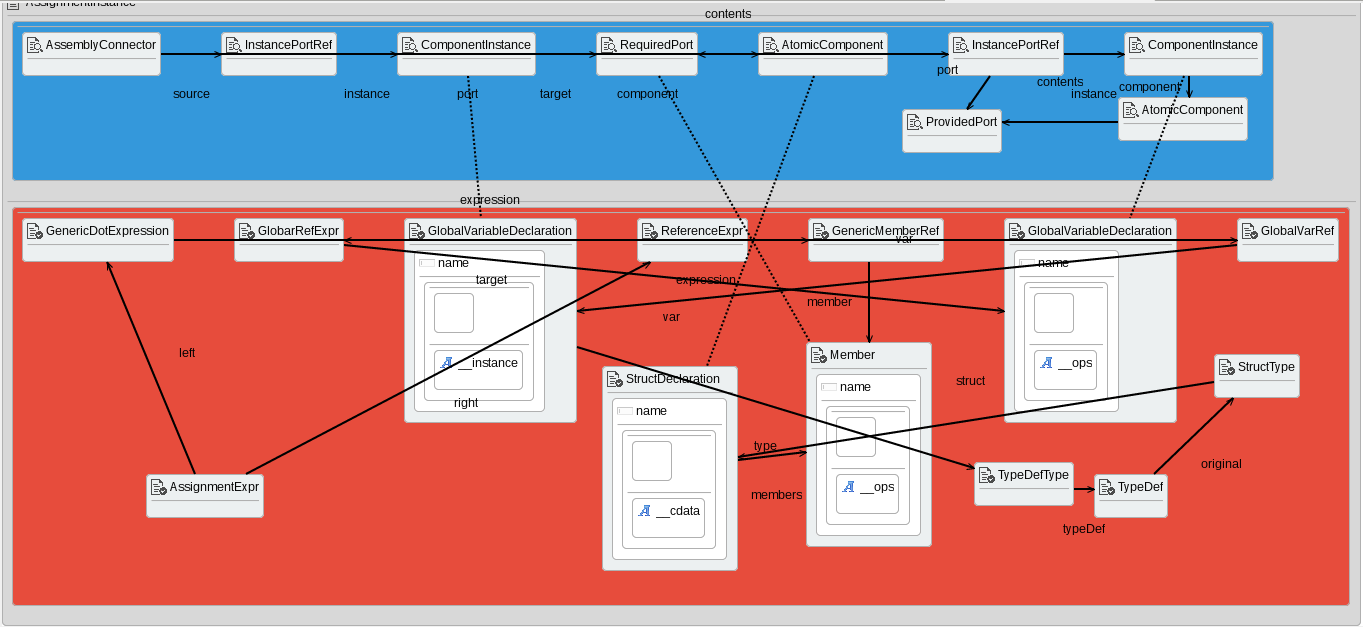
\includegraphics[width=0.48\textwidth]{figures/mbeddr/contracts/AssignmentInstance}
  \caption{AssignmentInstance contract}
  \label{fig:assignment_instance}
\end{center}
\end{figure}

Figure~\ref{fig:assignment_instance} shows the AssignmentInstance contract. This contract...

\subsection{Contract 2: GlobalVar}

\begin{figure}
\begin{center}
  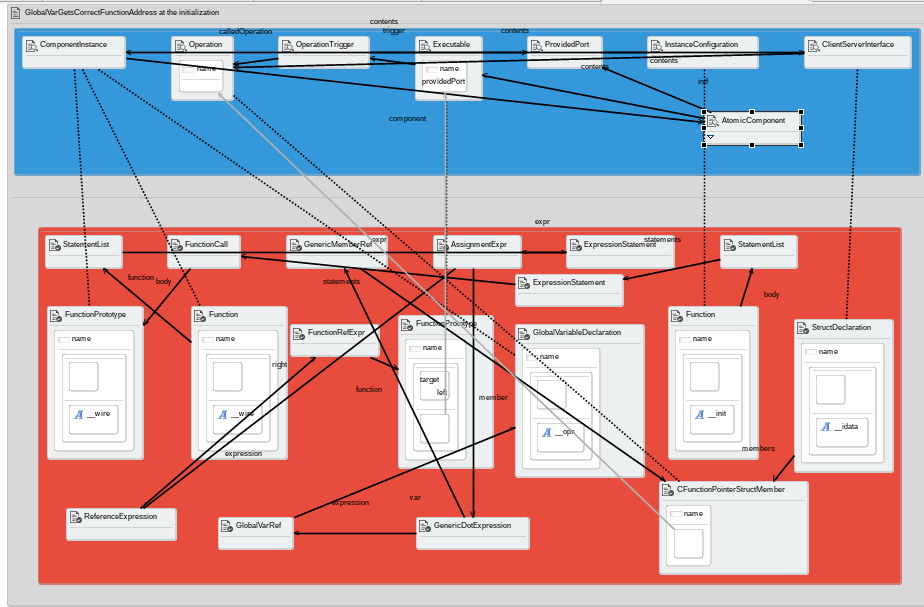
\includegraphics[width=0.48\textwidth]{figures/mbeddr/contracts/GlobalVar}
  \caption{GlobalVar contract}
  \label{fig:global_var}
\end{center}
\end{figure}

Figure~\ref{fig:global_var} shows the GlobalVar contract. This contract...

\subsection{Contract Discussion}

Note that there are a number of limitations on what can be verified on this transformation. First, due to the symbolic execution nature of the approach, it is not possible to verify instance data. For example, that all components have a valid name. Second, it is difficult if not impossible to validate semantic properties, such as...




















